% Canonical caption for figClassSizeLadder.pdf
% Generated by: code/module_c/cs_figures.py from
% code/figures/module_c/class_size/registered/cs_primary.csv
% and cs_projection.csv
\begin{figure}[tbp]
  \centering
  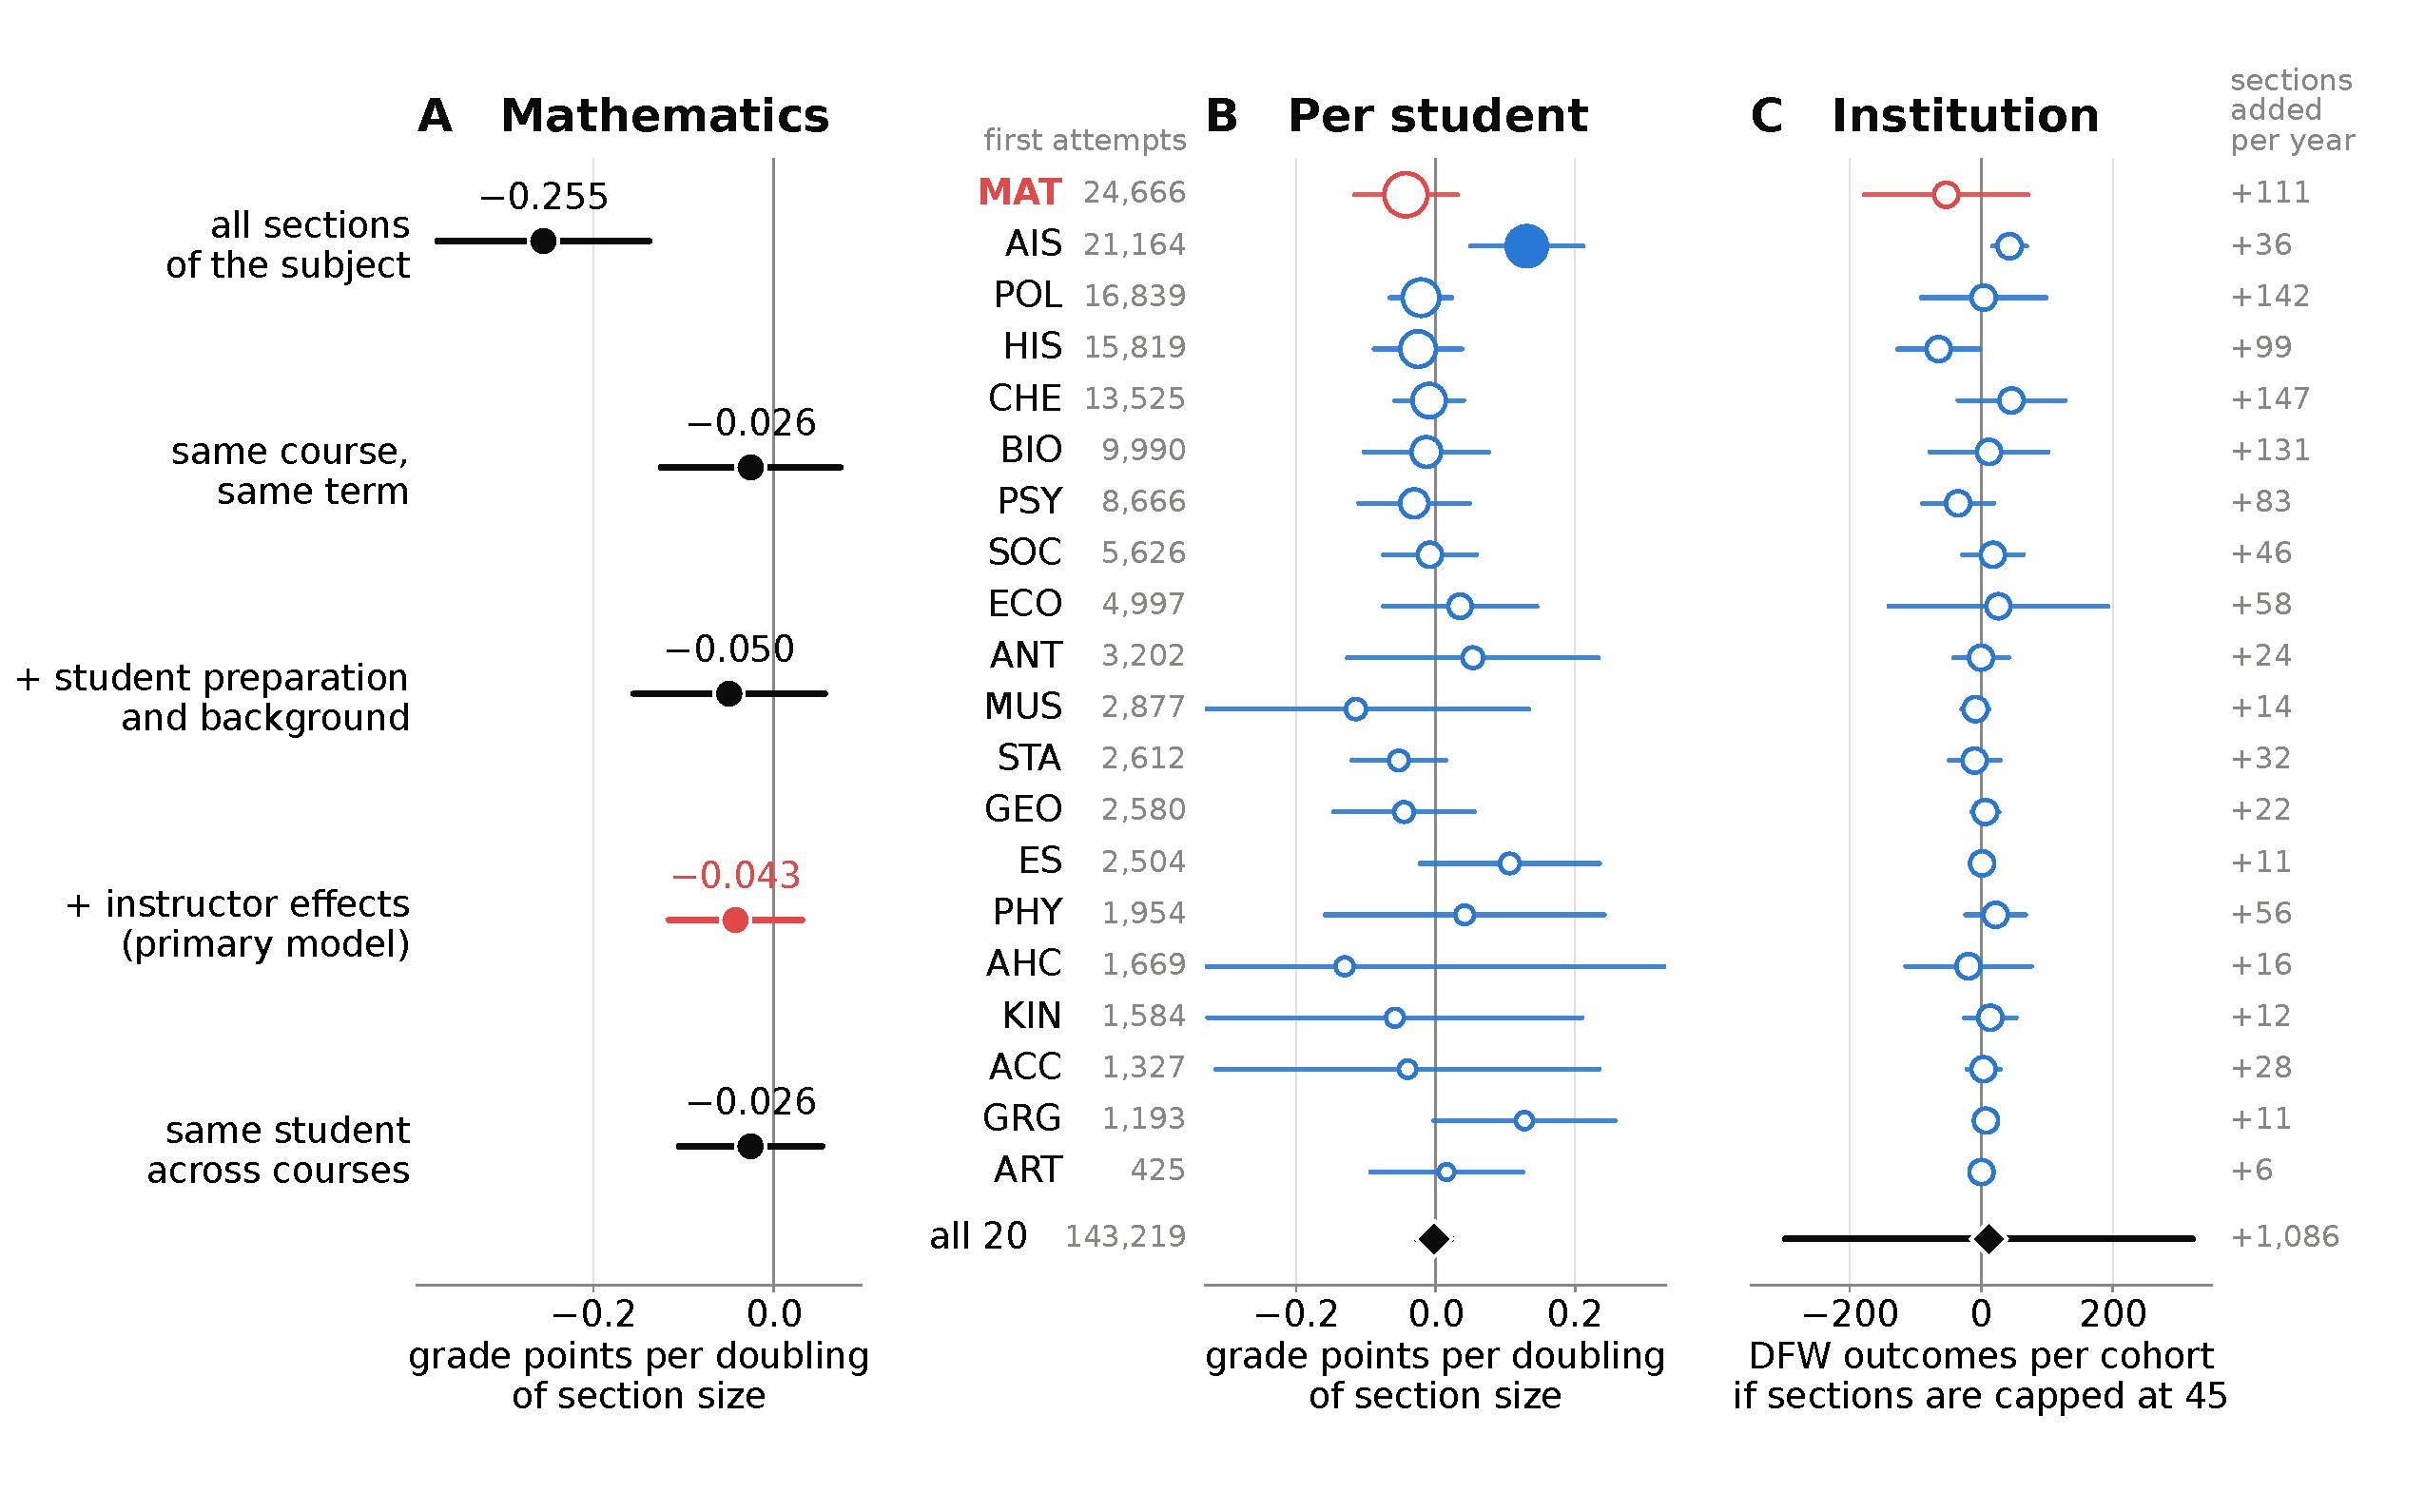
\includegraphics[width=0.95\textwidth]{figClassSizeLadder.pdf}
  \caption{Section size and first-attempt outcomes among
    first-time fall entrants of Fall 2014 to Fall 2018 in
    face-to-face lecture sections of more than 10 students.
    Intervals are 95\%, from a wild cluster bootstrap over
    instructors (the same-student row uses instructor-clustered
    standard errors). (A) Mathematics
    (24,666 first attempts, 18,878
    students, 1,040 sections,
    73 instructors): the difference in
    grade points that goes with a doubling of section size as the
    comparison tightens. Across all sections of the subject the
    coefficient is $-0.255$; with course-by-term effects, the
    student covariates, and instructor effects (the prespecified
    primary model, red), it is $-0.043$
    ($-0.117$ to $+0.031$; $p=0.258$), and the
    matching difference in the DFW rate is $+1.0$
    percentage points ($-1.3$ to
    $+3.3$). The last row compares each student
    with the same student in other courses. (B) The primary
    coefficient in each of 20 subjects, ordered by the
    first attempts each serves (printed beside the code, from
    24,666 in MAT to 425 in ART), with
    marker area proportional to that count; filled markers pass
    false-discovery control at $q=0.05$
    (1 of 20). The diamond is the random-effects
    pooled estimate, $-0.002$ ($-0.026$ to $+0.022$), with an interval that includes the covariance between subject estimates. The axis is set by the 90th percentile of interval reach; 2 wider intervals run past it.
    (C) The same subjects on the scale of the institution: the
    projected change in DFW outcomes per entry cohort if every
    lecture section above 45 students were split (the
    scenario of Table~\ref{tab:classsizescenario}), which
    multiplies each subject's DFW coefficient by the first
    attempts affected and by the change in their section sizes;
    the lecture sections the split would add per year are printed
    at right.
    Mathematics: $-53$
    ($-178$ to
    $+71$); all 20
    subjects (diamond): $+12$
    ($-297$ to $+321$). No subject passes
    false-discovery control on the DFW coefficient. Every
    estimate is an association conditional on entry. Section
    assignment is administrative, and the projection of panel C
    applies only if the association is the effect of size. Subject
    codes: MAT, mathematics; AIS, the first-year seminar; POL, political science; HIS, history; CHE, chemistry; BIO, biology; PSY, psychology; SOC, sociology; ECO, economics; ANT, anthropology; MUS, music; STA, statistics; GEO, geology; ES, environmental science; PHY, physics; AHC, art history and criticism; KIN, kinesiology; ACC, accounting; GRG, geography; ART, art.}
  \label{figClassSizeLadder}
\end{figure}
